\chapter{The LHC and the CMS Detector}
\label{chap:cmsoverview}

Probing nature for signs of physics beyond the \ac{SM} would not be possible without the immensely complex electronics and machinery that has made the TeV energy scale accessible to physicists for the first time. This chapter will introduce both the \ac{lhc} based at \acf{CERN}  and the \acf{CMS} detector (of which the author is a member). Section (\ref{sec:cmsdetector}) serves to present an overview of the different components of  the \ac{CMS} detector, with specific components relevant to the search for supersymmetric particles described in greater detail. Section (\ref{sec:cmsobjects}) will focus on particle and kinematic object reconstruction, again, with more emphasis on jet level quantities which are most relevant to the author's analysis research.

\section{The LHC}
\label{sec:thelhc} 

The \ac{lhc} is a storage ring, accelerator, and collider of circulating beams of protons or ions. Housed in the tunnel dug for the \acf{LEP}, it is approximately 27 km in circumference, 100 m underground, and straddles the border between France and Switzerland, outside of Geneva. It is currently the only collider in operation that is able to study physics at the TeV scale.  A double-ring circular synchrotron, it was designed to collide proton-proton (pp) pairs with a centre of mass energy of up to $\sqrt{s} = $ 14 \TeV at a final design luminosity of $10^{34}$cm$^{-2}$s$^{-1}$. \\

These counter-circulating beams of protons or Pb ions are merged in four sections around the ring to enable collisions of the beams, with each interaction point being home to one of the four major experiments; \acf{ALICE} \cite{alicetdr}, \acf{ATLAS} \cite{atlastdr}, the \acf{CMS} \cite{cmstdr} and \acf{LHCb} \cite{lhcbtdr} which record the resultant collisions. The layout of the \ac{lhc} ring is shown in Figure \ref{fig:lhc-ring}. The remaining four sections contain acceleration, collimation and beam dump systems. In the eight arc sections, the beams are steered by magnetic fields of up to 8 \T provided by super conduction dipole magnets, which are maintained at temperatures of 2 \K using superfluid helium. Additional magnets for focusing and corrections are also present in straight sections within the arcs and near the interaction regions where the detectors are situated. \\


\begin{figure}[!h]

\centering
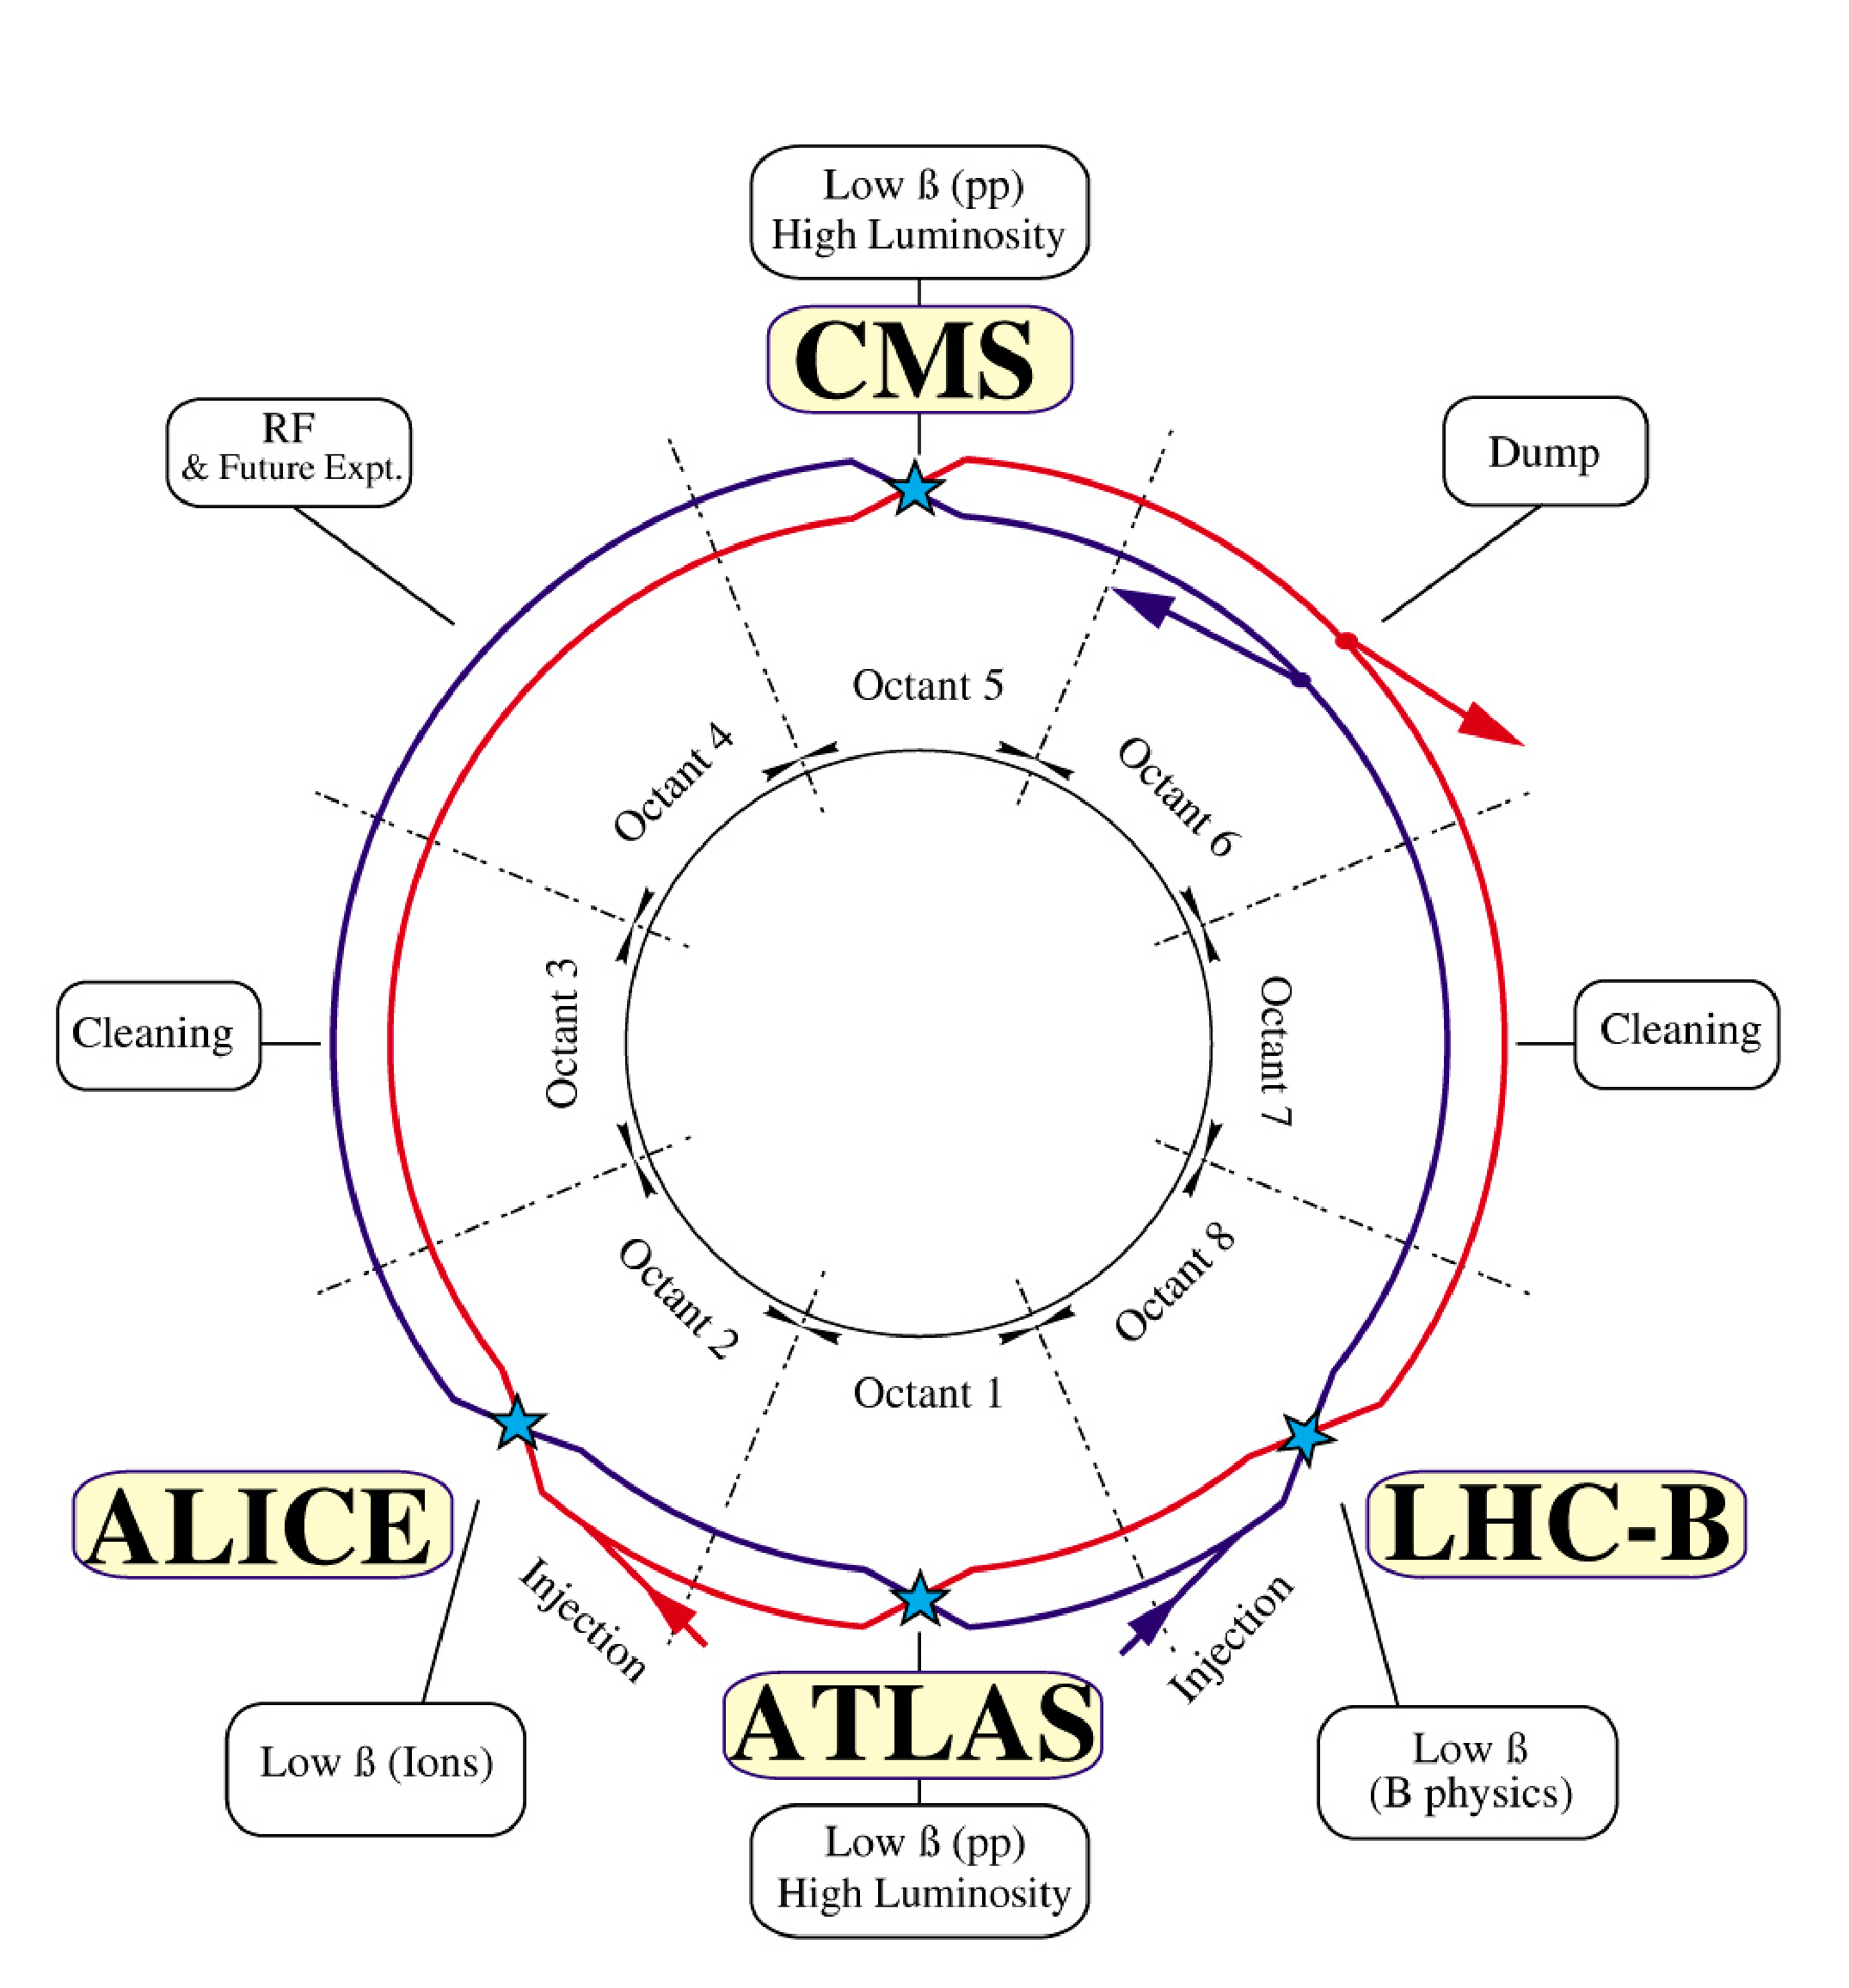
\includegraphics[width=0.60\textwidth]{plots/lhc-ring-photo.pdf}
\caption[A top-down layout of the \LHC, with the position of the four main detectors labelled.]{A top down layout of the \LHC. \cite{Jean-Luc:841573}, with the position of the four main detectors labelled.}  
\label{fig:lhc-ring}
\end{figure}


Proton beams are formed inside the \acf{PS} from bunches of protons 50 \ns apart with an energy of 26 \GeV. The protons are then accelerated in the \acf{SPS} to 450 \GeV  before being injected into the \ac{lhc}. These \ac{lhc} proton beams consists of many ``bunches" (i.e. approximately $1.1 \times 10^{11}$  protons localised into less than 1 \ns in the direction of motion).  Before collision, the beams are ramped to 4 \TeV (2012) per beam, in a process involving increasing the current passing through the dipole magnets. Once the desired \com energy is reached then the beams are allowed to collide at the interaction points. The luminosity falls regularly as the run progresses; protons are lost in collisions, and eventually the beam is dumped before repeating the process again. 

Colliding the beams produced an instantaneous peak luminosity of approximately 5 $\times$ 10$^{33}$ cm$^{-2}$s$^{-1}$ during the \com $=$ 8 \TeV run period in 2012. The high number of protons in each bunch increases the likelihood of multiple interactions with each crossing of the counter-circulating beams. This leads to isotropic energy depositions within the detectors positioned at these interaction points, increasing the overall energy scale of the collision. This is known as \emph{pile-up} and the counteracting of or correcting for its effects are important to the many measurements performed at the \ac{lhc}.

In the early phase of prolonged operation, after the initial shutdown, the machine operated in 2010-2011 at 3.5 \TeV per beam, \com $=$ 7 \TeV, delivering 6.13 \fb of data \cite{LHClumo}. During the 2012-2013 run period, data was collected at an increased \com $=$ 8 \TeV improving the sensitivity of searches for new physics. Over the whole run period 23.3 \fb of data was delivered, of which 21.8 \fb was recorded by the \ac{CMS} detector as shown in Figure \ref{fig:lhc-lumo} \cite{LHClumo}. A total of 12 \fb of certified data was collected by October 2012. Results within this thesis are presented utilising only this dataset as it formed the basis of the most recent journal publication in which the author was a significant contributor. 

\begin{figure}[!h]
\centering
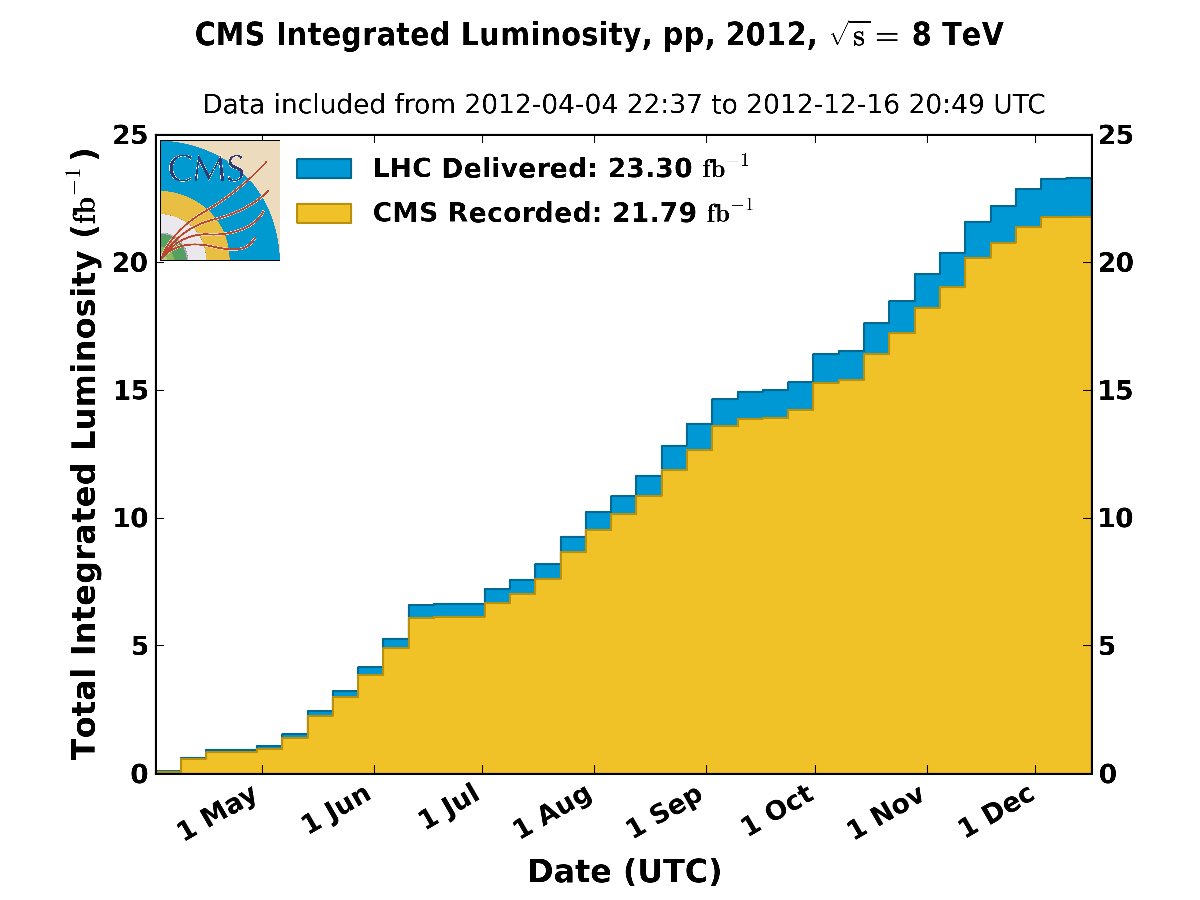
\includegraphics[width=0.60\textwidth]{plots/lhc-lumo-8tev.pdf}
\caption[The total integrated luminosity delivered to and collected by \ac{CMS} during the 2012 8 \TeV \pp runs]{The total integrated luminosity delivered to and collected by \ac{CMS} during the 2012 8 \TeV \pp runs.}  
\label{fig:lhc-lumo}
\end{figure}


\section{The CMS Detector}
\label{sec:cmsdetector}

The \acf{CMS} detector is one of two general purpose detectors at the \ac{lhc} designed to search for new physics. The detector is designed to provide efficient identification and measurement of many physics objects including photons, electrons, muons, taus, and hadronic showers over wide ranges of transverse momentum and direction. Its nearly 4$\pi$ coverage in solid angle allows for accurate measurement of global transverse momentum imbalance. These design factors give \ac{CMS} the ability to search for direct production of \ac{SUSY} particles at the \TeV scale, making the search for Supersymmetric particles one of the highest priorities among the wide range of physics programmes at \ac{CMS}. 

\ac{CMS} uses a right-handed Cartesian coordinate system with the origin at the interaction point and the z-axis pointing along the beam axis. The x-axis points radially inwards to the centre of the collider ring, with the y-axis pointing vertically upward. The azimuthal angle $\phi$, ranging between [$-\pi$,$\pi$], is defined in the x-y plane starting from the x-axis. The polar angle $\theta$ is measured from the z axis. The common convention in particle physics is to express an out-going particle in terms of $\phi$ and its pseudorapidity defined as

\begin{equation}
\eta = -\log\tan\left(\frac{\theta}{2}\right).
\end{equation}

In hadron collider physics, pseudorapidity is preferred over the polar angle \theta to describe particles trajectory because, the differences in pseudorapidity between outgoing particles are invariant under boosts along the z axis. 

The variable $\Delta R = \sqrt{\Delta\phi^{2} + \Delta\eta^{2} } $ is commonly used to define angular distance between objects within the detector. Additionally, energy and momentum is typically measured in the transverse plane perpendicular to the beam line. This is used because, whilst the initial longitudinal momentum in a parton collision is unknown, it is however known that the initial transverse momentum was zero. These values are calculated from the x and y components of the object and are denoted as $\et = E\sin\theta$ and $\pt = \sqrt{p^{2}_{x}+p^{2}_{y}}$. 

\subsection{Detector Subsystems}
\label{subsec:detectorsubsystems}

As the range of particles produced from \pp collisions interact in different ways with matter, \ac{CMS} is divided into sub-detector systems, which perform complementary roles in identifying, the mass and the momentum of different physics objects present in each event. These detector sub-systems contained within \ac{CMS} are wrapped in layers around a central 13m long 4 \T super conducting solenoid, as shown in Figure \ref{fig:cms-detector}. With the endcaps closed, \ac{CMS} is a cylinder of length 22m, diameter 15m, and mass 12.5 kilotons. A more detailed complete description of the detector can be found elsewhere \cite{cmstdr}. \\

\begin{figure}[!h]

\centering
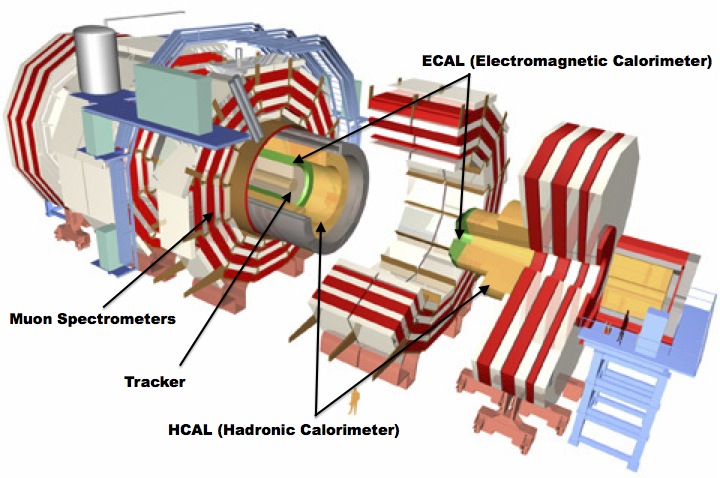
\includegraphics[width=0.65\textwidth]{plots/cms-detector.pdf}
\caption[A pictorial depiction of a cutaway of the \ac{CMS} detector.]{A pictorial depiction of a cutaway of the \ac{CMS} detector with the main detector subsystems used in particle identification labelled \cite{cms-public-detector}.}  
\label{fig:cms-detector}
\end{figure}

\subsection{Tracker}
\label{subsec:tracker}

 The inner-most sub-detector of the barrel is the multi-layer silicon tracker, formed of a pixel detector component encased by layers of silicon strip detectors. The pixel detector consists of three layers of silicon pixel sensors providing measurements of the momentum, position coordinates of the charged particles as they pass, and the location of primary and secondary vertices between 4 cm and 10 cm transverse to the beam. Outside the pixel detector, ten cylindrical layers of silicon strip detectors extend the tracking system out to a radius of 1.20m from the beam line. The tracking system provides efficient and precise determination of the charges, momenta, and impact parameters of charged particles, with the geometry of the tracker extending to cover a rapidity range up to $\lvert\eta\rvert \textless$ 2.5.  \\
 
 The tracking system also plays a crucial part in the identification of jets that originate from b-quarks through the measurement of displaced secondary vertices. The methods in which these b-flavoured jets are identified are discussed within Section (\ref{subsec:cmsobjects-btagging}). The identification of b-jets is important in many searches for natural \ac{SUSY} models and forms an important part of the inclusive search strategy described within Section (\ref{subsec:searchstrategy}).
 
\subsection{Electromagnetic Calorimeter}
\label{subsec:ecal}

 Immediately outside of the tracker, but still within the magnet core, sits the \acf{ECAL}. Covering a pseudorapidity up to $\lvert\eta\rvert < 3$ and comprising of over 75 $\times 10^{3}$ PbWO$_{4}$ (lead tungstate) crystals that scintillate as particles deposit energy in them, the \ac{ECAL} provides high resolution measurements of the electromagnetic showers from photons and electrons in the detector. \\ 
 
 Lead tungstate is used because of its short radiation length ($X_{0} \sim 0.9$ cm) and small Molier\'{e} radius ($\sim 2.1$ cm) leading to high granularity and resolution. Its fast scintillation time ($\sim 25$ ns) reduces the effects of pile-up, and its radiation hardness give it longevity. The crystals are arranged in modules which surround the beam line in a non-projective geometry,  angled at 3$^{\circ}$, with respect to the interaction point to minimise the risk of particles escaping down the cracks between the crystals.\\
 
 The  \ac{ECAL} is primarily composed of two sections, the \acf{EB} which extends in pseudo-rapidity to $\lvert\eta\rvert < 1.479$ with a crystal front cross section of 22$\times$22 mm and a length of 230 mm corresponding to 25.8 radiation lengths. The \acf{EE} covers a rapidity range of $1.479 < \lvert\eta\rvert < 3.0 $, which consists of two identical detectors
on either side of the \ac{EB}.  A lead-silicon sampling `pre-shower' detector \acf{ES} is placed before the endcaps to aid in the identification of neutral pions. Their arrangement is shown in Figure \ref{fig:cms-ecal}. \\

 
 \begin{figure}[!h]

\centering
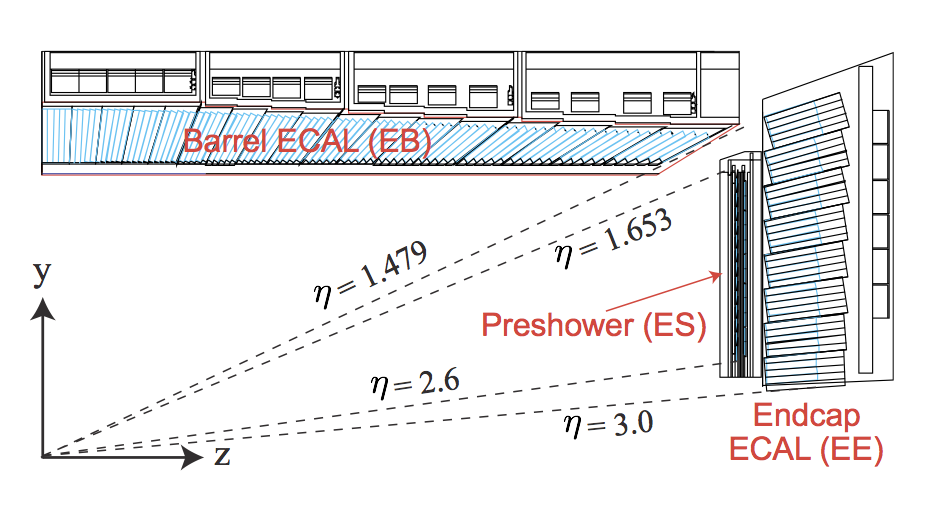
\includegraphics[width=0.85\textwidth]{plots/cms-ecal.pdf}
\caption[Illustration of the \ac{CMS} \ac{ECAL}. ]{Illustration of the \ac{CMS} \ac{ECAL} showing the arrangement of the lead tungstate crystals in the \ac{EB} and \ac{EE}. The \ac{ES} is also shown and is located in front of the \ac{EE} \cite{CMS_ECAL_TDR}. The $\eta$ segmentation of the \ac{ECAL} is also shown via dotted lines.}  
\label{fig:cms-ecal}
\end{figure}


Scintillation photons from the lead tungstate crystals are instrumented with \acf{APD} and \acf{VPT}, located in the \ac{EB} and \ac{EE} respectively. They convert the scintillating light into an electric signal which is consequently used to determine the amount of energy deposited within the crystal. These instruments are chosen for their resistance under operation to the strong magnetic field of \ac{CMS}. The scintillation of the \ac{ECAL} crystals, as well as the response of the \ac{APD}s, vary as a function of temperature; and so cooling systems continually maintain an overall constant \ac{ECAL} temperature $\pm 0.05 ^{\circ}$C.
 

\subsection{Hadronic Calorimeter}
\label{subsec:hcal} 

Beyond the \ac{ECAL} lies the \acf{HCAL} which is responsible for the accurate measurement of hadronic showers, crucial for analyses involving jets or missing energy signatures. The \ac{HCAL} is a sampling calorimeter which consists of alternating layers of brass absorber and plastic scintillator, the exception being in the hadron forward ($3.0 < \lvert\eta\rvert < 5.0 $) region where steel absorbers and quartz fibre scintillators are used because of their increased radiation tolerance. Hadron showers are initiated in the absorber layers inducing scintillation in the plastic scintillator tiles.  These scintillation photons in the blue-violet region of the spectrum spectrum are then absorbed and re-emitted at longer wavelengths by wavelength shifting fibres for more efficient read-out by hybrid photodiodes. \\

The \ac{HCAL}'s size is constrained to a compact size by the presence of the solenoid, requiring the placement of an additional outer calorimeter on the outside of the solenoid to increase the sampling depth of the \ac{HCAL}. A schematic of the \ac{HCAL} can be seen in Figure \ref{fig:cms-hcal}.\\
 
 \begin{figure}[!h]

\centering
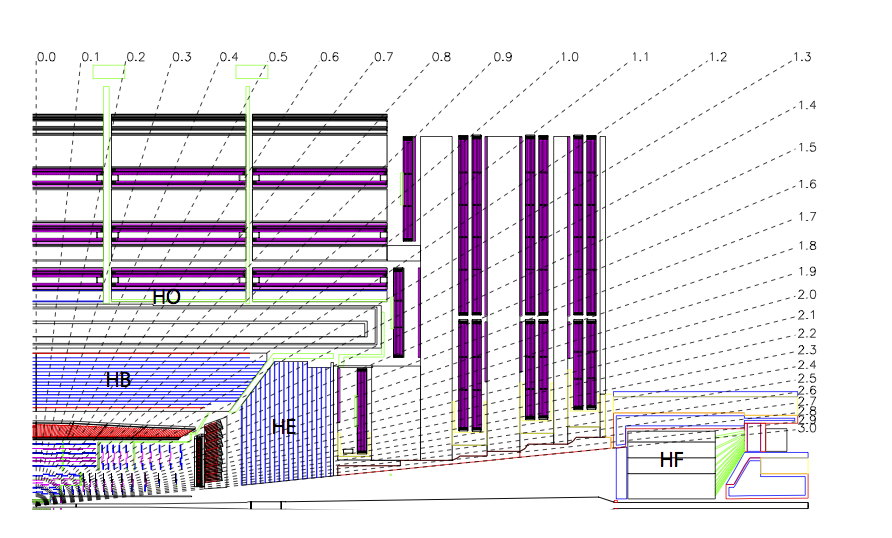
\includegraphics[width=0.85\textwidth]{plots/cms-hcal.pdf}
\caption[Schematic of the \ac{CMS} \acf{HCAL}.]{ Schematic of the hadron calorimeters in the r-z plane, showing the locations of the \ac{HCAL} components and the \ac{HF}. Other detector subsystems are also displayed for scale, with the $\eta$ segmentation of the \ac{CMS} detector shown by the dotted lines \cite{cmstdr}.}  
\label{fig:cms-hcal}
\end{figure}
 
The \ac{HCAL} covers the range $\lvert\eta\rvert < 5$ and consists of four sub-detectors: the \ac{HB}  $\lvert\eta\rvert < 1.3$, the \acf{HO}, the \acf{HE} $1.3 < \lvert\eta\rvert < 3.0 $ and the \acf{HF}.  The \ac{HB}, contained between the outer edge of the \ac{ECAL} and the inner edge of the solenoid is formed of 36 azimuthal wedges which are split between two half-barrel segments. Each wedge is segmented into four azimuthal angle ($\phi$) sectors, and each half-barrel is further segmented into 16 $\eta$ towers. The electronic readout chain channels the light from the active scintillator layers from one $\phi$-segment and all $\eta$-towers of a half-barrel to a \acf{HPD}.

The relatively short number of interaction lengths, $\lambda_{l}$,  within the \ac{HB} justifies the need for the `tail catching' \ac{HO} to increase the sampling depth in the central barrel rapidity region $\lvert\eta\rvert < 1.3$. This gives a total sampling depth of up to 11 interaction lengths in the central region. 

Significant fractions of a hadron's energy will also be deposited in the \ac{ECAL} from its decay into lighter particles as it passes through the detector. Therefore, measurements of hadron energies in the central regions $\lvert\eta\rvert < 3.0$ use both the \ac{ECAL} and \ac{HCAL} to reconstruct the true energy from showering hadrons. 

\subsection{Muon Systems}
\label{subsec:muonsystems} 
 
Muons being too massive to radiate away energy via Bremsstrahlung, mostly pass through the detector until they reach the system of muon detectors which forms the outer-most part of the \ac{CMS} detector.  

Outside of the superconducting solenoid are four muon detection layers interleaved with the iron return yokes, which measure the muons energy via ionisation of gas within detector elements. Three types of gaseous chambers are used. The \acf{DT}, \acf{CSC}, and \acf{RPC} systems provide efficient detection of muons with pseudo-rapidity $\lvert\eta\rvert < 2.4 $. The best reconstruction performance is obtained when the muon chamber is combined with the inner tracking information to determine muon trajectories and their momenta \cite{CMS_MUON_TDR}.  \\ 

\subsection{Triggering System}

\label{sec:triggersystem}

Bunch crossings at the \ac{lhc} during the \com = 8 \TeV run were separated by just 50 ns. Therefore the rate at which data from all collisions would have to be stored on disk and subsequently processed would be unfeasible. A two-tiered triggering system is applied at \ac{CMS} in order to cope with the high collision rate of protons. The \ac{CMS} trigger is designed to use limited information from each event to determine whether to record it, reducing the rate of data taking to manageable levels whilst ensuring a high efficiency of interesting physics object events are selected.

The \ac{L1} is a pipelined, dead-timeless system based on custom-built electronics \cite{Sphicas:2002gg}, and is a combination of several sub systems which is shown pictorially in Figure \ref{fig:l1triggersystem}. This figure shows that the \L1 trigger is itself split into two subsystems, the \acf{GCT} and the \acf{GMT} which form calorimeter or muon objects from the combination of information from their own respective detector subsystems.

The \L1 system is covered in more detail within the following chapter, along with a description benchmarking the performance of the \L1 calorimeter trigger during the \com = 8 \TeV run period.

\begin{figure}[ht]
\centering
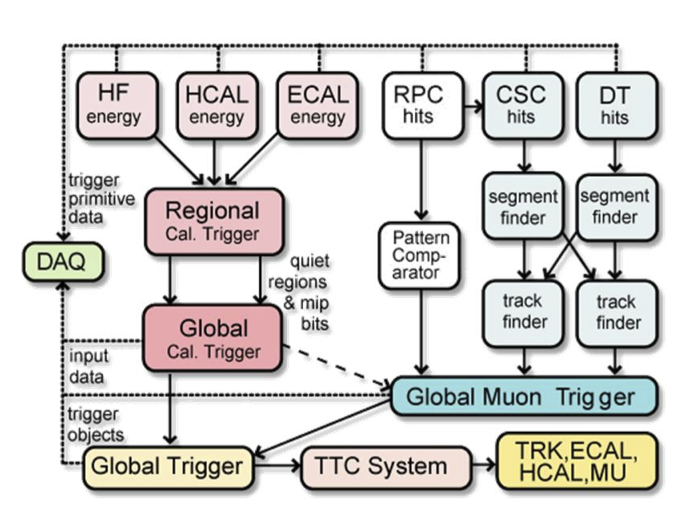
\includegraphics[width=0.75\textwidth]{plots/l1triggersystem.pdf}
\caption[An overview of the different components of the \ac{CMS} \L1 trigger system]{An overview of the different components of the \ac{CMS} \L1 trigger system, showing the global calorimeter, muon triggers, and the global trigger.}  
\label{fig:l1triggersystem}
\end{figure}

The \acf{HLT} is a large farm of commercial computers \cite{Sphicas:2002gg}. The \ac{HLT} processes events with software reconstruction algorithms that are more detailed, giving performance more similar to the reconstruction used offline. The \ac{HLT} reduces the event rate written to disk by a factor of $\sim$ 500 ($\sim$200Hz). The recorded events are transferred from \ac{CMS} to the \ac{CERN} computing centre, where event reconstruction is performed, and then distributed to \ac{CMS} computing sites around the globe for storage and analysis.



\section{Event Reconstruction and Object Definition}
\label{sec:cmsobjects}

The goal of event reconstruction is to take the information from the coordinates and magnitudes of energy deposits recorded by the detector and to compute from it higher-level quantities which can be used at an analysis level. These typically correspond to an individual particle's identity and its energy and momenta, groups of particles which shower in a narrow cone, and the overall global energy and momentum balance of the event. 

Covered within this section is a brief introduction to jet reconstruction and the identification of jets originating from a b-quark, which are very relevant to the analysis detailed in Chapter \ref{chap:SUSYsearches}. Additionally, the identification criteria for the selection of muon, electron, photon and jet objects used by each of the analyses described within this thesis are also introduced within the following section. A much deeper discussion of the reconstruction of all physics objects used by \ac{CMS} can be found in \cite{CMS_TDR_PHYS_vol1}.

\subsection{Jets}
\label{subsec:cmsobjects-jets}

Quarks and gluons are produced copiously at the LHC in the hard scattering of partons. As these quarks and gluons fragment, they hadronize and decay into a group of strongly interacting particles and their decay products. These streams of particles travel in the same direction away from interaction point, as they have been ``boosted" by the momentum of the primary hadron. These collections of decay products are reconstructed and identified together as a ``jet''.

At \ac{CMS} jets are reconstructed from energy deposits in the detector via the anti-kt algorithm \cite{antiktalgo} with size parameter $\Delta R = 0.5$. The anti-kt jet algorithm clusters jets by defining a distance between hard (high-$\pt$) and soft (low-$\pt$) particles such that soft particles are preferentially clustered with hard particles before being clustered between themselves. This produces jets which are robust to the pile-up conditions produced from proton-proton collisions at the \ac{lhc}. 

There are two main types of jet reconstruction used at \ac{CMS}, Calorimeter (\Calo) and Particle Flow (\PF) jets \cite{CMS-PAS-JME-10-003}. Calorimeter jets are reconstructed using both the \ac{ECAL} and \ac{HCAL} cells, combined into ``calorimeter towers''. These calorimeter towers consist of geometrically matched groups of \ac{HCAL} cells and \ac{ECAL} crystals. Electronics noise in each cell is suppressed by applying a threshold to the calorimeter cells, with pile-up effects reduced by a requirement placed on the tower energy  \cite{Janssen:1322145}. Calorimeter jets are the jets used within the analysis presented in this thesis, due to the computational time required to construct \PF jets and the use of these reconstructed jets within the \ac{HLT} trigger paths of the analysis.   

\PF jets are formed from combining information from all of the \ac{CMS} sub-detectors systems to  determine which final state particles are present in the event. Generally, any particle is expected to produce some combination of a track in the silicon tracker, a track in the muon system and/or a deposit in the calorimeters. The \PF jet momentum and spatial resolutions are greatly improved with respect to calorimeter jets, as the use of the tracking detectors and of the high granularity of \ac{ECAL} allows resolution and measurement of charged hadrons and photons inside a jet,  which together constitute $\sim$ 85$\%$ of the jet energy \cite{1748-0221-6-11-P11002}.

The jets reconstructed by the clustering algorithm in \ac{CMS} typically have an energy that differs to the `true' energy measured by a perfect detector. This stems from the non-linear and nonuniform response of the calorimeters as well as other residual effects including pile-up and underlying events. Therefore, additional corrections are applied to recover a uniform relative response as a function of pseudo-rapidity. These are applied as separate sub corrections \cite{1742-6596-404-1-012014}. 

\begin{itemize}

\item A pile-up correction is first applied to the jet. It subtracts the average extra energy deposited in the jet that comes from other vertices present in the event and is therefore not part of the hard jet itself.
\item $\pt$- and $\eta$- dependent corrections derived from Monte Carlo simulations are used to account for the non-uniform response of the detector.\item $\pt$- and $\eta$- residual corrections are applied to data only to correct for difference between data and Monte Carlo simulations. The residual is derived from QCD di-jet samples and the $\pt$ residual from $\gamma + $ jet and $Z + $ jets samples in data.

\end{itemize}

\subsection{B-tagging}
\label{subsec:cmsobjects-btagging}

The decays of b-quarks are suppressed by small \CKM matrix elements. As a result, the lifetimes of b-flavoured hadrons, produced in the fragmentation of b-quarks, are relatively long; $\sim$1ps. Therefore these hadrons can fly a significant distance in the detector before decaying, giving rise to displaced vertices within the jet. The identification of jets originating from b-quarks is very important for searches for new physics and for measurements of \ac{SM} processes.  \\

Several different algorithms developed by \ac{CMS} select b-quark jets based on variables such as; the impact parameters of the charged-particle tracks, the properties of reconstructed decay vertices, and the presence or absence of a lepton, or combinations thereof. 

One of the most efficient algorithms is the \acf{CSV} algorithm \cite{CMS-PAS-BTV-09-001}. This operates based on secondary vertex and track-based lifetime information, benchmarked in `Loose', `Medium' and `Tight' working points, corresponding to the mis-identi�cation probability for light-parton jets of 10$\%$, 1$\%$, and 0.1$\%$, respectively, in jets with an average $\pt$ of about 80 \GeV. Light parton jets are defined as those which originate from a u, d, s quark or a gluon. The medium working point is used within the \alphat search presented in Section (\ref{sec:alphatintroduction}), which is measured to have a gluon/light-quark tagging efficiency of $\sim$ 1\%, a c-quark tagging efficiency of $\sim$ 20\% and a jet p$_{\text{T}}$ dependant b-tagging efficiency of 60-70\% \cite{btagscalefactor}.


Within the \ac{CSV} tagger, a likelihood-based discriminator distinguishes between jets from b-quarks, and those from charm or light quarks and gluons, the distribution of which is shown in Figure \ref{fig:btagdescrims}. All figures within this sub-section, demonstrating the performance of this b-tagging algorithm are taken from \cite{CMS-PAS-BTV-13-001}.

\begin{figure}[ht]
\centering
\begin{minipage}[b]{0.70 \linewidth}
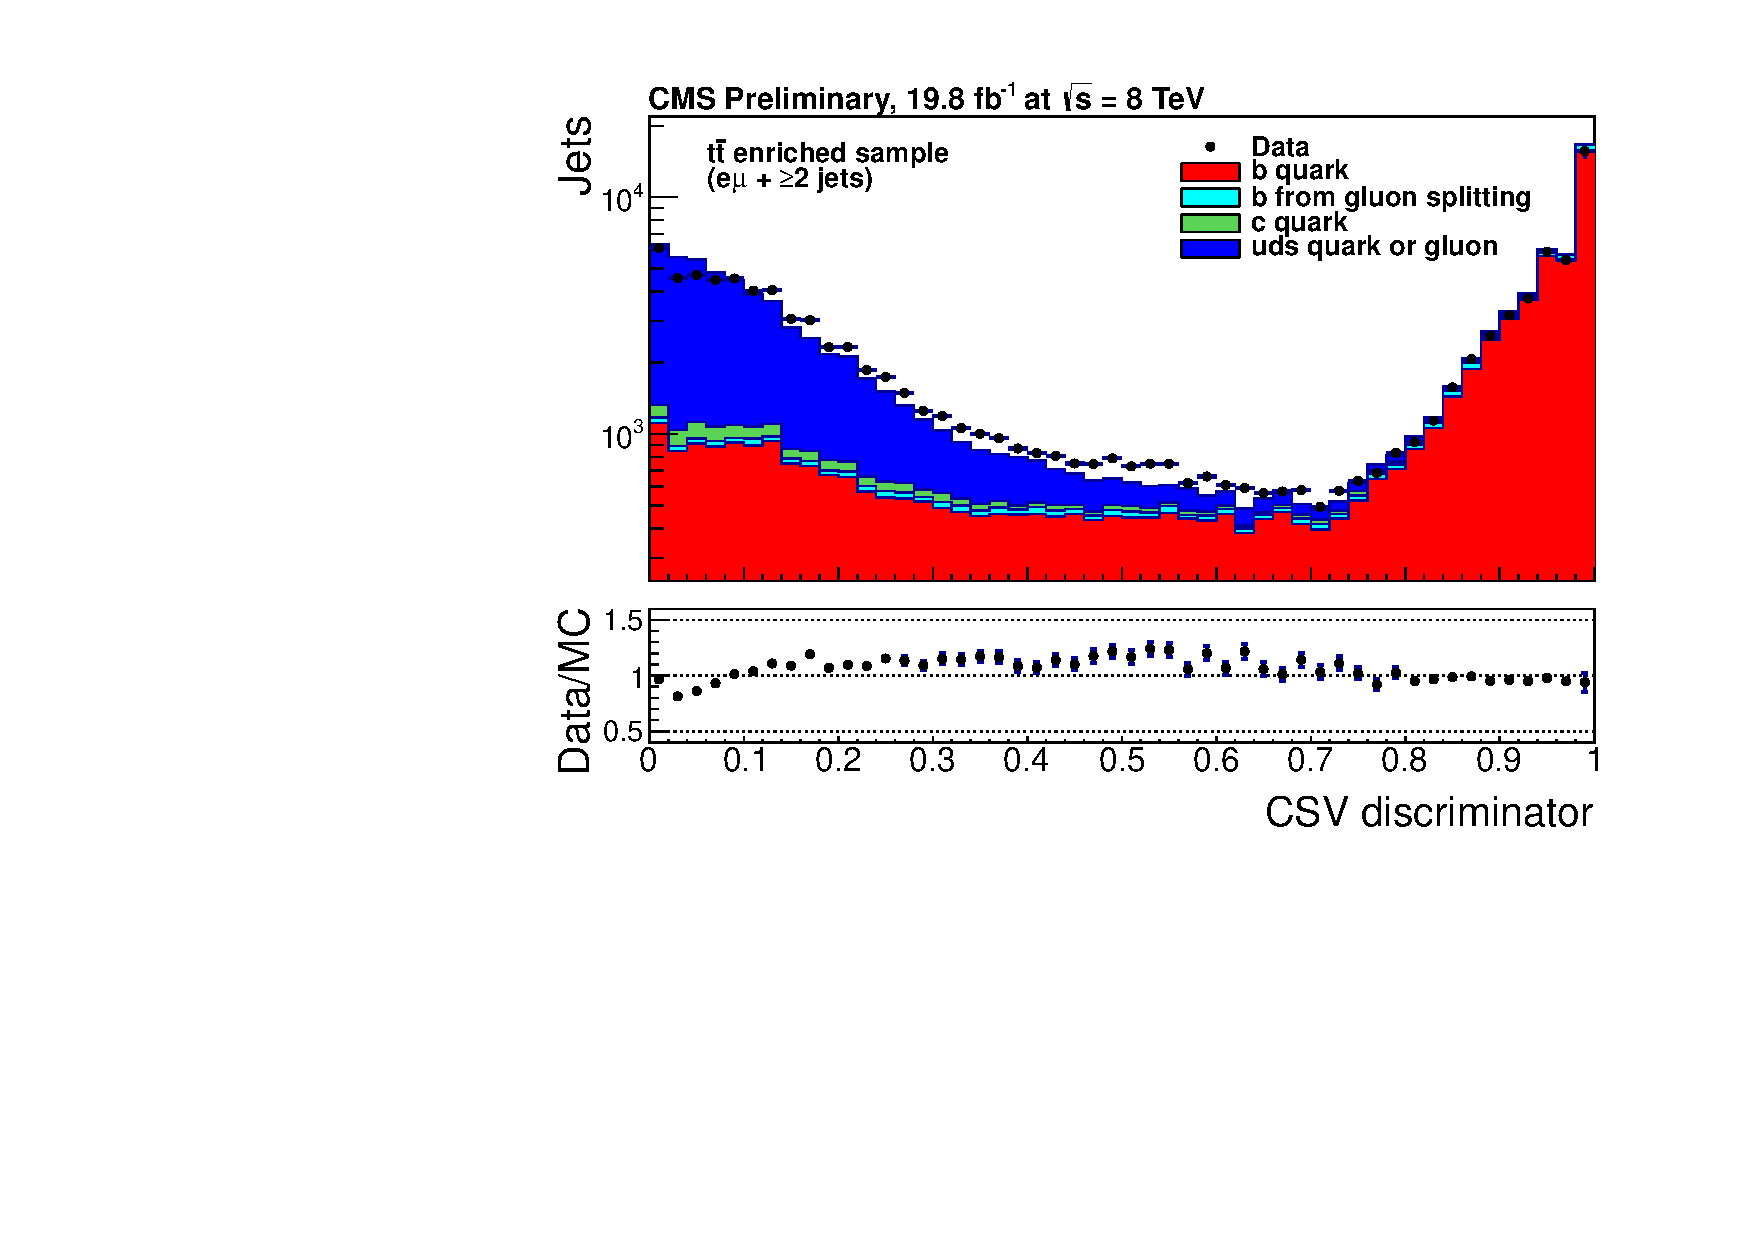
\includegraphics[width = 1.0\linewidth]{plots/btag-ttbardiscrim.pdf}
\end{minipage}
\quad
\begin{minipage}[b]{0.70\linewidth}
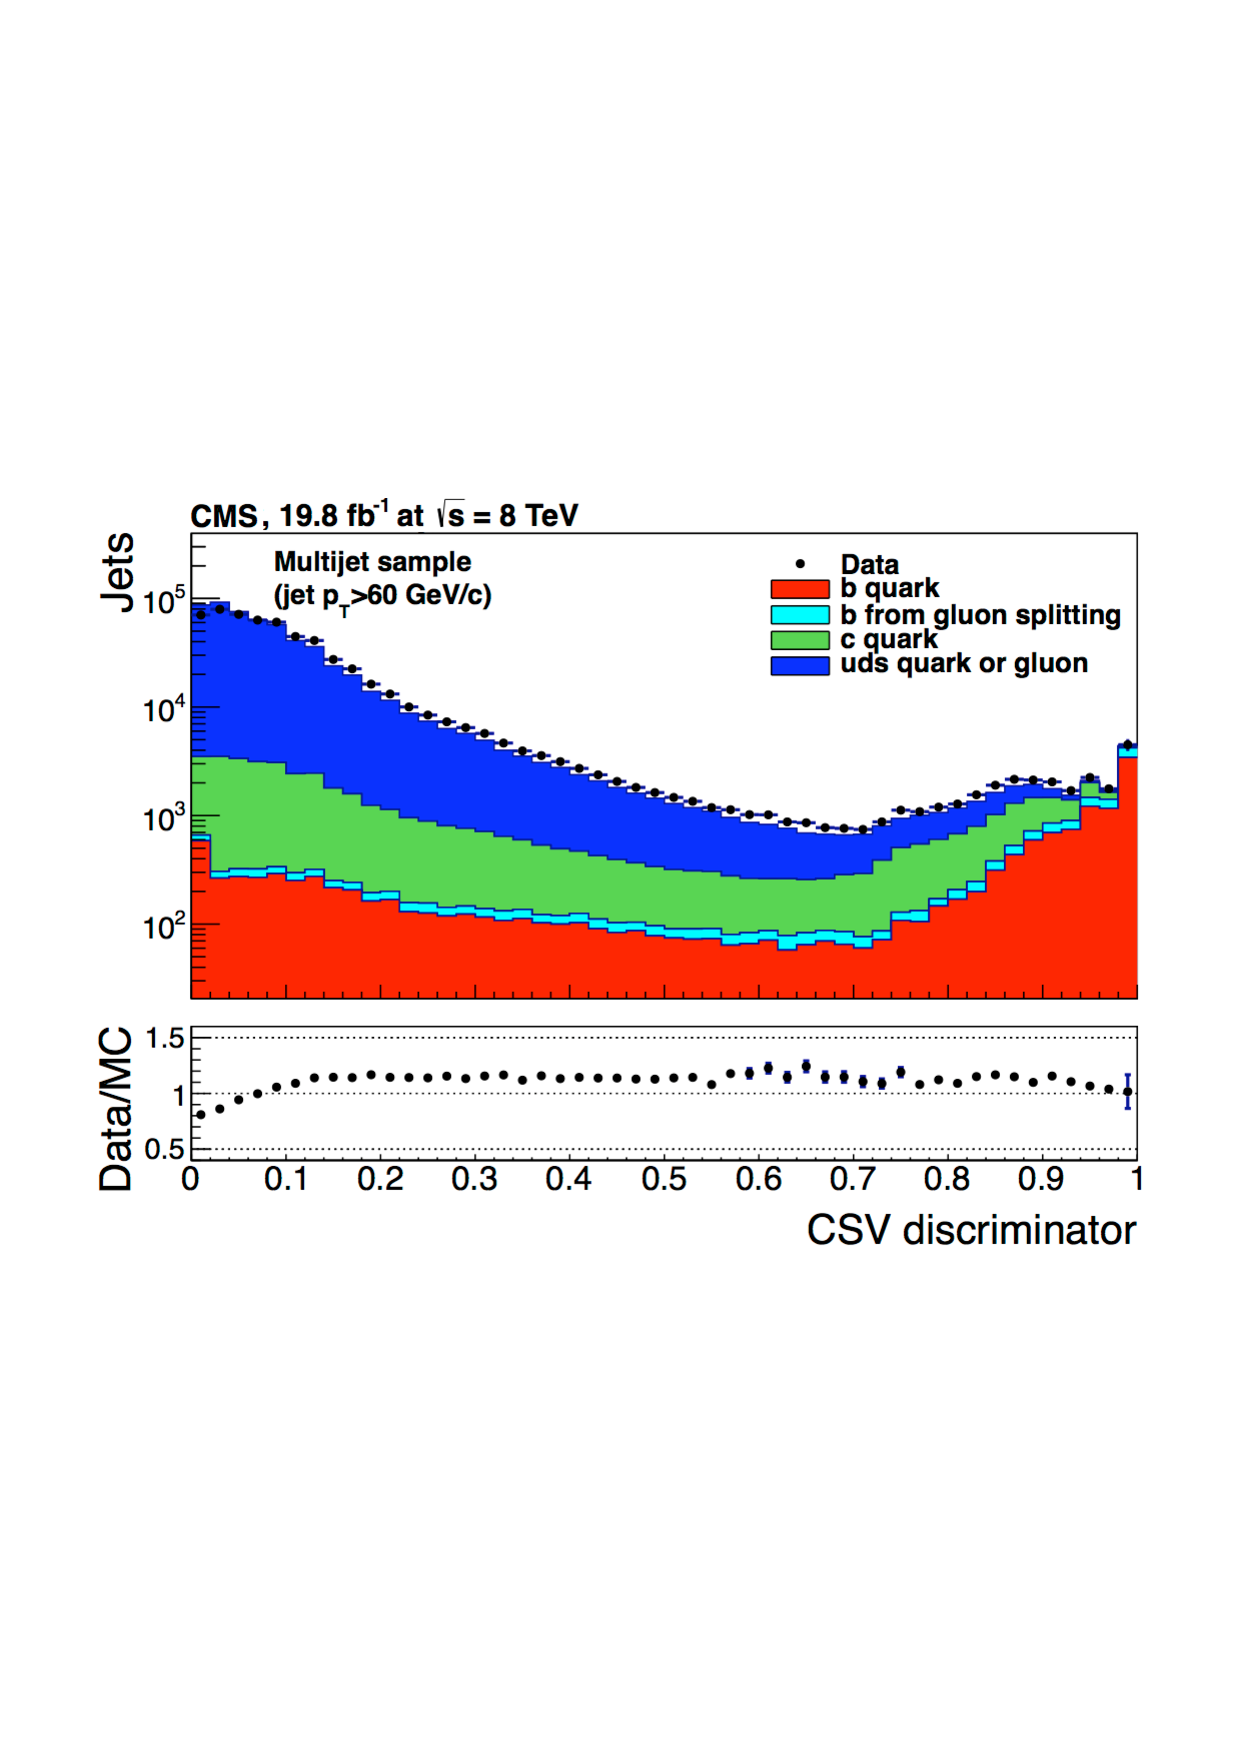
\includegraphics[width = 1.0\linewidth]{plots/btag-multijetdiscrim.pdf}
\end{minipage}
\caption[ \ac{CSV} algorithm discriminator values in enriched ttbar and inclusive multi-jet samples]{\ac{CSV}algorithm discriminator values in enriched ttbar (top) and inclusive multi-jet samples (bottom) for b,c and light flavoured jets. The discriminator value used for each working points are determined from the misidentification probability for light-parton jets to be tagged as a b-jet, which are given as 0.244 (10\%), 0.679 (1\%) and 0.898 (0.1\%) for the L, M and T working points respectively \cite{CMS-PAS-BTV-13-001}. }
\label{fig:btagdescrims}
\end{figure}

The b-tagging performance is evaluated to measure the b-jet tagging efficiency \effb, and the misidentification probability of charm \effc and light-parton jets \effs . The tagging efficiencies for each of these three jet flavours are compared between data and MC simulation, from which a series of $\pt$ and $\lvert\eta\rvert$ dependant jet corrections are determined,

\begin{equation}
SF_{b,c,s} = \frac{\epsilon^{data}_{b,c,s}}{\epsilon^{MC}_{b,c,s}} .
\end{equation}

The variables $\epsilon^{data}_{b,c,s}$ and $\epsilon^{MC}_{b,c,s}$ correspond to the efficiency as measured in data or simulation for jets originating from a b-quark, c-quark of light parton respectively. 

These are collectively named `B-tag Scale Factors' and allow MC simulation to accurately reflect the running conditions and performance of the tagging algorithm in data. A good understanding of the tagging efficiency for each of the jet flavours is essential in order to minimise systematic uncertainties in physics analyses that employ b-tagging. \\
 
The b-tagging efficiency is measured in data using several methods applied to multi-jet events, primarily based on a sample of jets enriched in heavy flavour content. One method requires the collection of events with a poorly isolated muon within a cone $\Delta R < 0.4$ around the jet axis. Due to the semi-leptonic branching fraction of b hadrons being significantly larger than that for other hadrons, these jets are more likely to arise from b quarks than from another flavour. The resultant momentum component of the muon, transverse to the jet axis, is larger in b-hadron decays than from light or charm flavoured jets.  

Additionally, the performance of the tagger can also be benchmarked in \ttbar events, where the top quark is expected to decay to a W boson and a b quark about 99.8$\%$ of the time \cite{pdg2012}. Further selection criteria is applied to these events to further enrich the b quark content of these events. The methods to identify b-jets in data are discussed in greater detail at \cite{btag7tev}. The jet flavours within simulation are determined using truth level information which is spatial matched to reconstructed jets, and is then compared to measurements in data to determine an appropriate set of $\pt$- and $\lvert\eta\rvert$- dependent scale factors ($SF_{b,c,s}$). The scale factor corrections from simulation to data for b-quark jets determined for the \ac{CSVM} tagger are displayed in Figure \ref{fig:btagscalefactors}. 

\begin{figure}[ht]
\centering
\begin{minipage}[b]{0.44\linewidth}
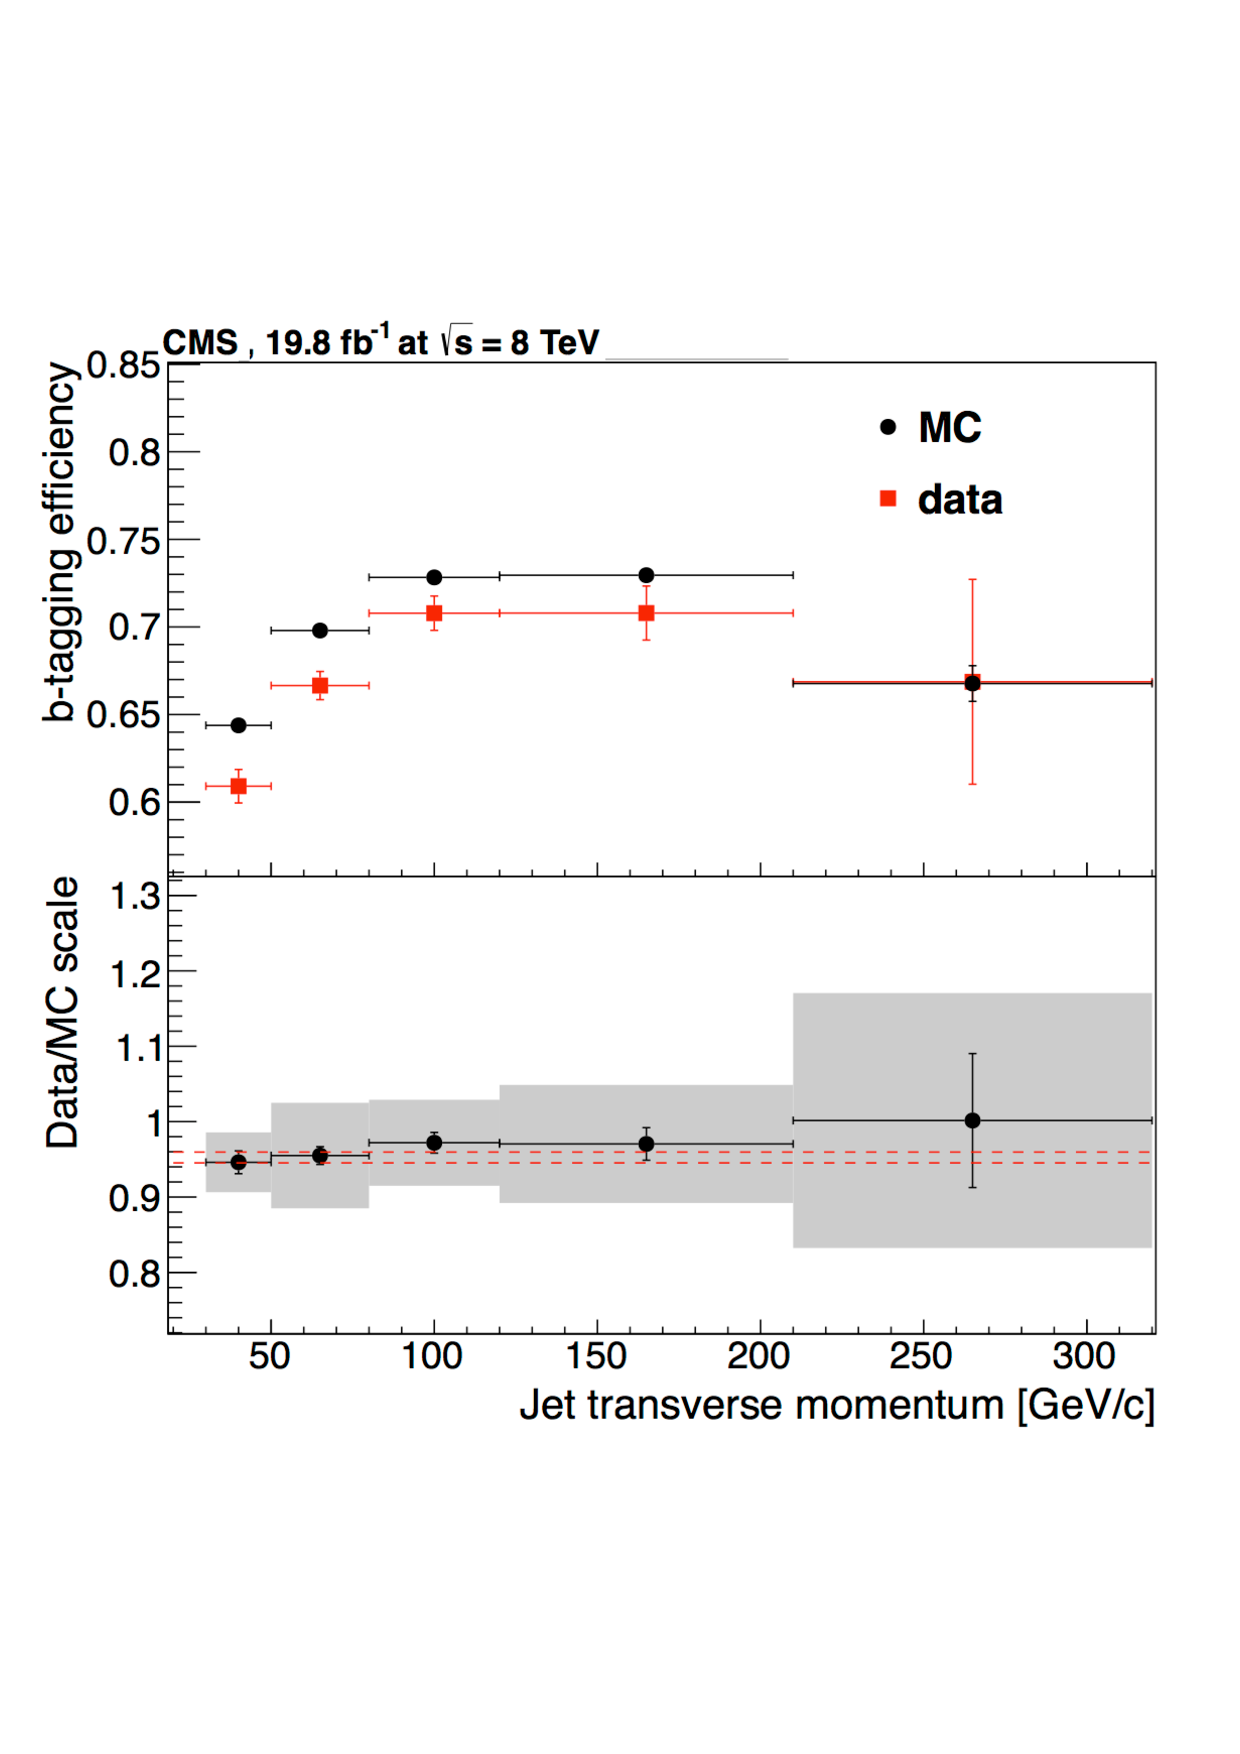
\includegraphics[width = 1.0\linewidth]{plots/btag-csvm_pt_sf.pdf}
\end{minipage}
\quad
\begin{minipage}[b]{0.44\linewidth}
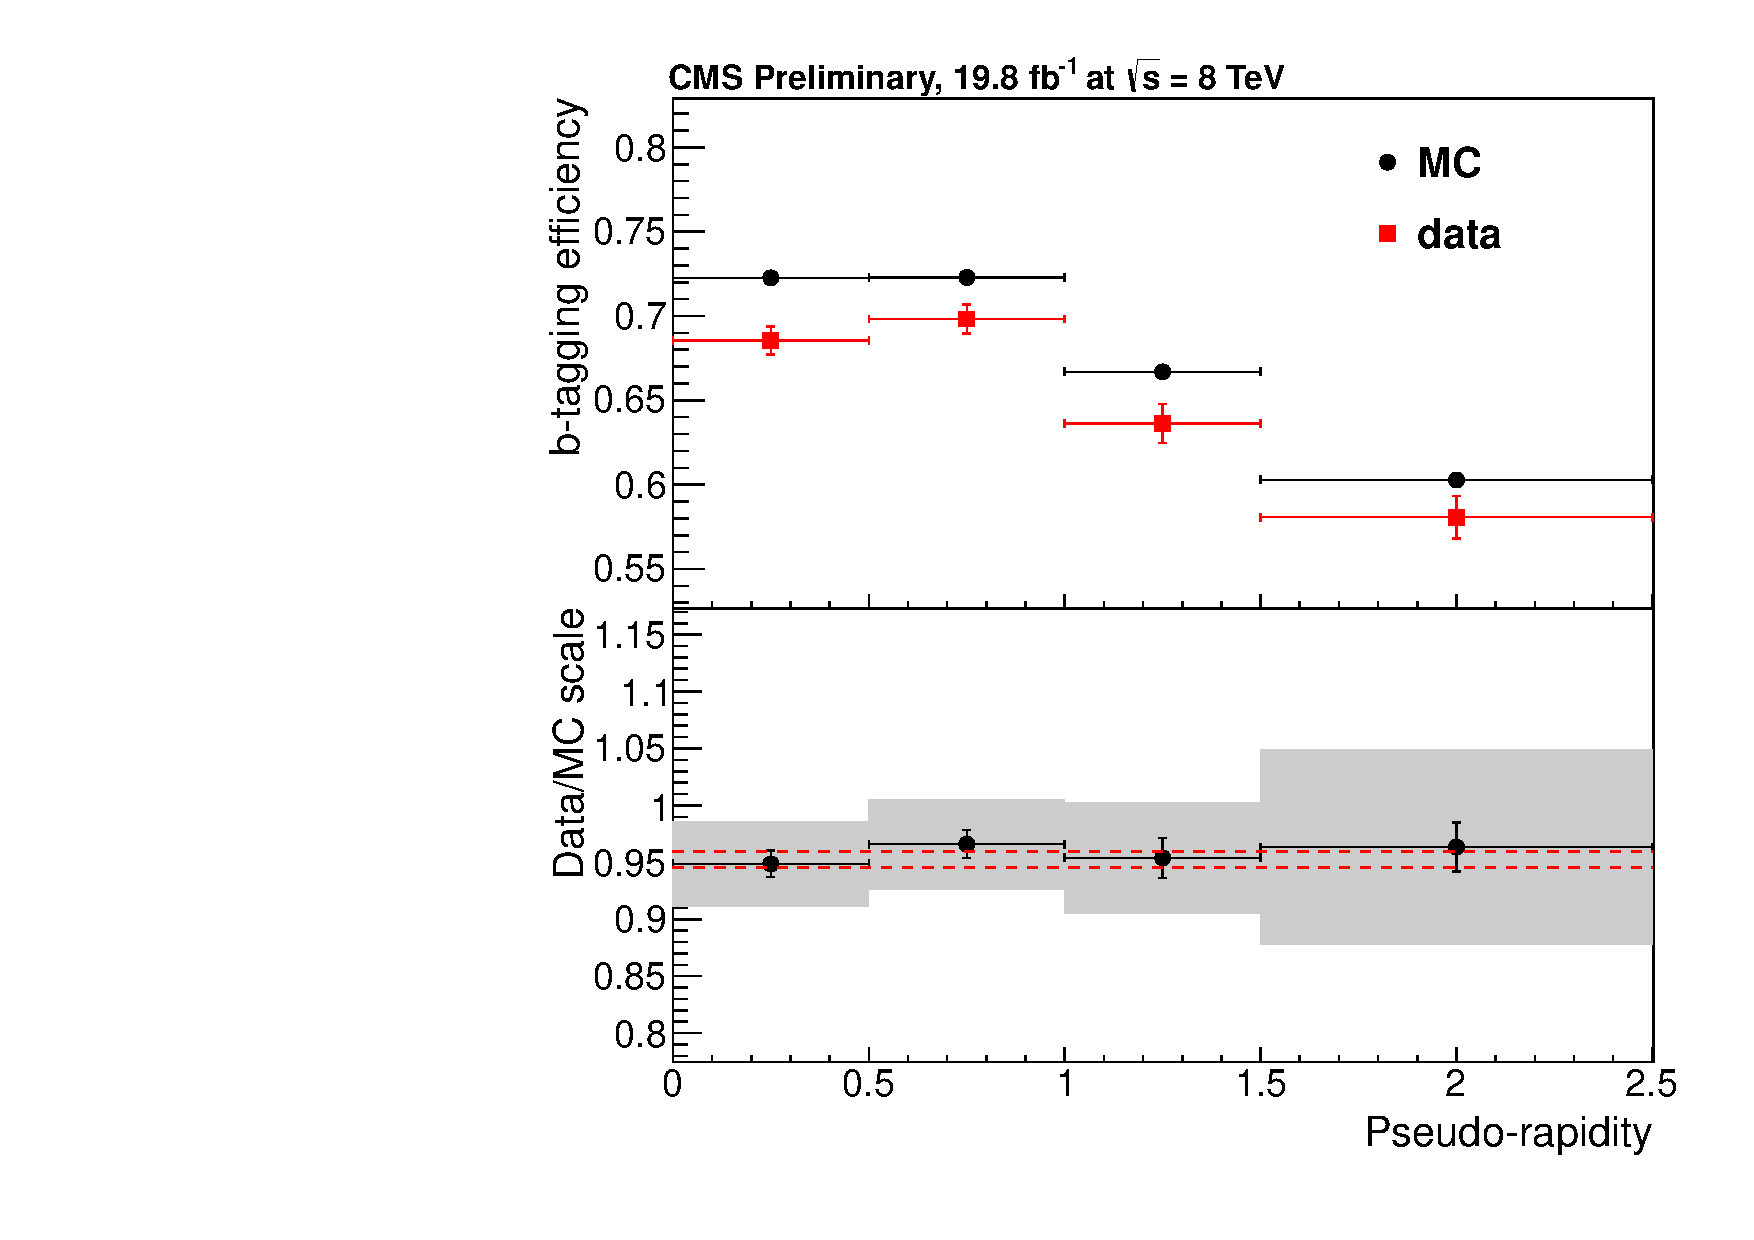
\includegraphics[width = 1.0\linewidth]{plots/btag-csvm_eta_sf.pdf}
\end{minipage}
\caption[Data/MC b-tag scale factors derived using the \ac{CSVM} tagger.]{Measured in \ttbar $\rightarrow$ di-lepton events using the \ac{CSVM} tagger: (upper panels) b-tagging efficiencies and (lower panels) data/MC scale factor $SF_{b}$ as a function of (left) jet $\pt$ and (right) jet $\lvert\eta\rvert$. In the lower panels, the grey filled areas represent the total statistical and systematic uncertainties, whereas the dotted lines are the average $SF_{b}$ values within statistical uncertainties \cite{CMS-PAS-BTV-13-001}.}
\label{fig:btagscalefactors}
\end{figure}

The measurement of the misidenti�cation probability for light-parton jets relies on the inversion of tagging algorithms, selecting jets not having properties typical of b-jets using the same variables and techniques used for benchmarking the b-tagging efficiency. The scale factors ($SF_{s}$) determined as a function of jet \pt to correct Monte Carlo simulation to measurements in data are shown in Figure \ref{fig:mistagscalefactors} for the \ac{CSVM} tagger.

\begin{figure}[ht]
\centering
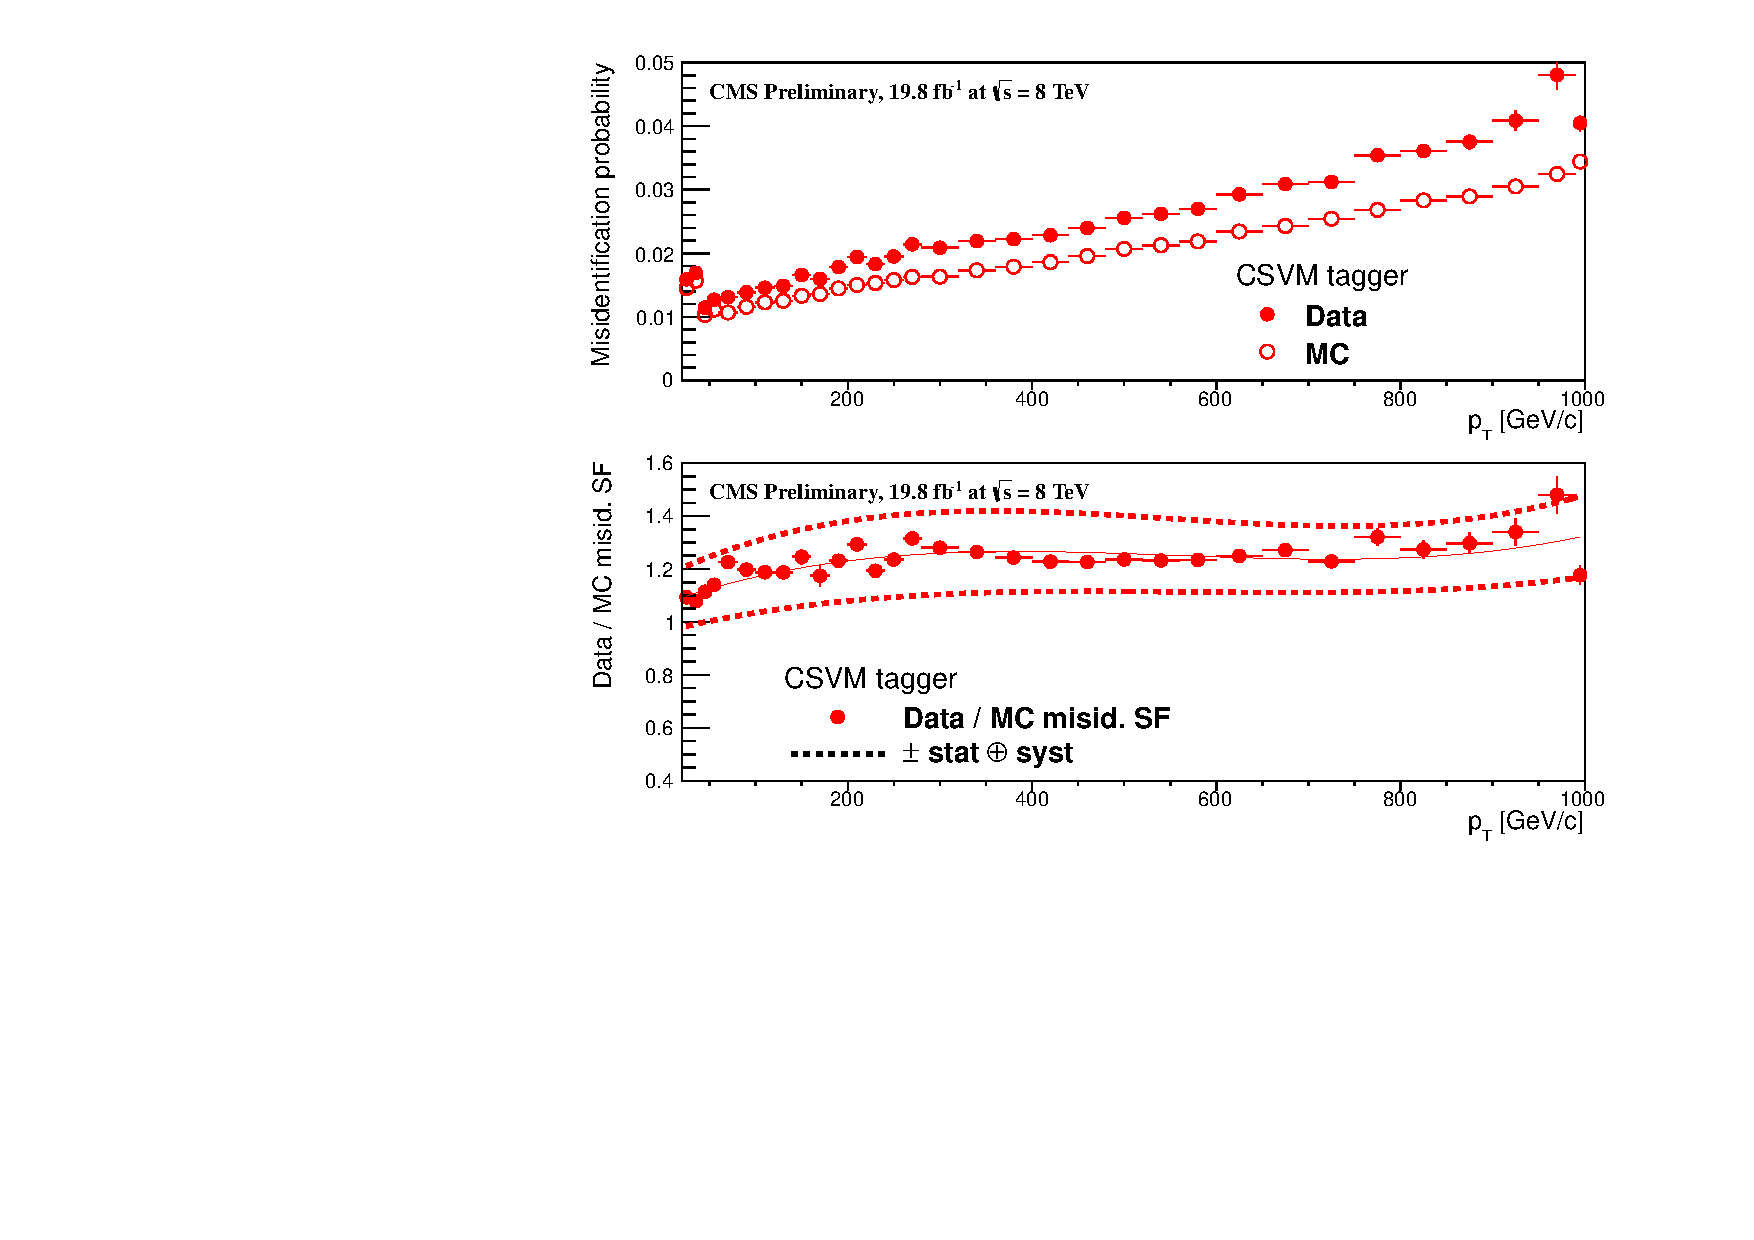
\includegraphics[width=0.70\linewidth]{plots/mistag_csvm.pdf}
\caption[Data/MC mis-tag scale factors derived using the \ac{CSVM} tagger.]{For the \ac{CSVM} tagging criterion: (top) misidenti�cation probability in data (filled circles) and simulation (open circles); (bottom) scale factor for the misidenti�cation probability. The last $\pt$ bin in each plot includes all jets with $\pt > 1000$ \GeV. The solid curve is the result of a polynomial fit to the data points. The dashed curves represent the overall statistical and systematic uncertainties on the measurements \cite{CMS-PAS-BTV-13-001}.}  

\label{fig:mistagscalefactors}
\end{figure}

\FloatBarrier

\subsection{Physics Analysis Objects}
\label{subsec:physicsobjects}

The physics objects used in the analyses described in this thesis are introduced below, and follow the recommendation of the various \ac{CMS} \acf{POGs}. 

\begin{itemize}

\item \textbf{Jets}

The jets used in the supersymmetric searches presented in this thesis are CaloJets, reconstructed as described earlier in this Section using the anti-k$_{T}$ jet clustering algorithm. 

To ensure the jet object falls within the calorimeter systems a pseudo-rapidity requirement of \abeta $<$ 3 is applied. Each jet must pass a ``loose'' identification criteria to reject jets resulting from unphysical energy, the criteria of which are detailed in Table \ref{tab:calojetid} \cite{CMS-PAS-JME-09-008}.

\begin{table}[H]
\footnotesize
\begin{center}
\begin{tabulary}{0.80\textwidth}{LL}
\cline{1-2}
\multicolumn{2}{l}{Loose CaloJet Id} \\
Variable & Definition \\ 
\hline\hline
f$_{HPD} < 0.98$ \qquad\qquad\qquad\qquad\qquad\qquad & Fraction of jet energy contributed from ``hottest'' \ac{HPD}, which rejects \ac{HCAL} noise.  \\
f$_{EM} > 0.01$ & Noise from the \ac{HCAL} is further suppressed by requiring a minimal electromagnetic component to the jet f$_{EM}$. \\
N$^{90}_{hits} \geq$ 2 & Jets that have $>$ 90\% of its energy from a single channel are rejected, to serve as a safety net that catches jets arising from undiagnosed noisy channels.\\
\hline
\end{tabulary}
\end{center}
\caption[Criteria for a reconstructed jet to pass the loose calorimeter jet id.]{Criteria for a reconstructed jet to pass the loose calorimeter jet id.}
\label{tab:calojetid}
\end{table}

\PF jets are used in the measuring the performance of the \L1 trigger, which is described in Chapter \ref{subsec:l1trigger}. These jets are identified wight he following criteria:
  
\begin{table}[H]
\footnotesize
\begin{center}
\begin{tabulary}{0.80\textwidth}{p{3.5cm}L}
\cline{1-2}
\multicolumn{2}{l}{Loose PF jet Id} \\
Variable & Definition \\ 
\hline\hline
nfhJet $<$ 0.99 & Fraction of jet composed of neutral hadrons. \ac{HCAL} noise tends to populate high values of neutral 
hadron fraction.\\
nemfJet $<$ 0.99 & Fraction of jet composed of neutral electromagnetic energy. \ac{ECAL} noise tends to populate high values of 
neutral EM fraction. \\
nmultiJet $>$ 1 & Number of constituents that jet is composed from. \\
chfJet $>$ 0 & Fraction of jet composed of charged hadrons. \\
cmultiJet $>$ 0 & Number of charged particles that compose jet. \\
cemfJet $<$ 0.99 & Fraction of jet composed of charged electromagnetic energy. \\
\hline
\end{tabulary}
\end{center}
\caption[Criteria for a reconstructed jet to pass the loose PF jet id.]{Criteria for a reconstructed jet to pass the loose PF jet id.}
\label{apptab:pfjetid}
\end{table}  


\item \textbf{Muons}

Muons are selected and vetoed in the control samples and signal region of the \alphat search in Chapter \ref{chap:SUSYsearches}. The following cut based selection is summarised in Table \ref{tab:muonidtable} and is used to identify muons in both instances with a 95$\%$ efficiency \cite{2012JInst...7P0002T}.

\begin{table}[h!]
\footnotesize
\begin{center}
\begin{tabulary}{0.98\textwidth}{LL}
\cline{1-2}
Variable & Definition \\ 
\hline\hline
Is Global Muon \qquad\qquad\qquad\qquad\qquad\qquad\qquad\qquad\qquad\qquad\qquad& Muon contains both a hit in the muon chamber and a matched track in the inner tracking system.\\
$\chi^{2}$$<$ 10 & $\chi^{2}$ of global muon track fit. Used to suppress hadronic punch-through and muons from decays in flight.  \\
Muon chamber hits $>$ 0 &  At least one muon chamber hit included in global muon track fit.\\
Muon station hits $>$ 1 & Muon segment hits in at least two muon stations, which  suppresses hadronic punch-through and accidental track-to-segment matches. \\
d$_{xy} <$ 0.2mm & The tracker track transverse impact parameter w.r.t the primary vertex. Suppresses cosmic muons and muons from decays in flight. \\
d$_{z} <$ 0.5mm & The longitudinal distance of the tracker track w.r.t the primary vertex. Loose selection requirement to further suppress cosmic muons, muons from decays in flight and tracks from pile-up.\\
Pixel hits $>$ 0 & Suppresses muons from decays in flight by requiring at least one pixel hit in the tracker. \\
Track layer hits $>$ 5 & Number of tracker layers with hits, to guarantee a good \pt measurement. Also suppresses muons from decays in flight.\\
PF Iso  $<$0.12 & Isolation based upon the sum of the charged and neutral hadrons and photon objects within a $\Delta$R 0.4 cone of the muon object, corrected for pile up effects on the isolation sum.   \\
\cline{1-2}
\end{tabulary}
\end{center}
\caption[Muon identification criteria used within the analysis for selection/veto purposes in the muon control/signal selections.]{Muon identification criteria used within the analysis for selection/veto purposes in the muon control/signal selections.}
\label{tab:muonidtable}
\end{table}
\FloatBarrier

Additionally muons are required to be within the acceptance of the muon tracking systems. Where the muon object is used in the triggering of the event, a \abeta $<$ 2.1 restriction is employed. In instances where muons are vetoed, a \abeta $<$ 2.5 and a minimum \pt $> 10 $ \GeV threshold requirement is placed on the identification of muon objects. 

\item \textbf{Photons} 

Photons are identified according to the cut based criteria listed in Table \ref{tab:photonidtable}, corresponding to 95$\%$ efficiency in the identification of genuine isolated photon objects \cite{CMS-PAS-SUS-12-018}.

\setlength\LTleft{1.5cm}
\setlength\LTright{\LTleft}
\begin{footnotesize}
\begin{center}
\begin{longtable}{@{\extracolsep{\fill}}p{2.0cm}p{10cm}}

\hline \multicolumn{2}{r}{\textit{Continued on next page}} \\ 
\endfoot

\endlastfoot
\hline
Variable & Definition \\ 
\hline\hline \\
H/E $< $ 0.05  & The ratio of hadronic energy in the \ac{HCAL} tower directly behind the \ac{ECAL} super-cluster and the \ac{ECAL} super-cluster itself. \\
$\sigma_{i\eta i\eta}< 0.011$ & The log energy weighted width ($\sigma$), of the extent of the shower in the $\eta$ dimension.\\
R9 $<$ 1.0 & The ratio of the energy of the 3$\times$3 crystal core of the super-cluster compared to the total energy stored in the 5$\times$5 super-cluster. \\
Combined Isolation $<$ 6 \GeV &  The photons are required to be isolated with no electromagnetic or hadronic activity within a radius $\Delta$R = 0.3 of the photon object. A combination of the pile-up subtracted (due to isotropic energy deposits) \cite{Cacciari:2007fd}, \ac{ECAL}, \ac{HCAL} and tracking isolation sums are used to determine the combined total isolation value.  \\
\hline
\caption[Photon identification criteria used within the analysis for selection/veto purposes in the \gpjets control/signal selections. ]{Photon identification criteria used within the analysis for selection/veto purposes in the \gpjets control/signal selections.}
\label{tab:photonidtable}
\end{longtable}
\end{center}
\end{footnotesize}

\FloatBarrier
Photon objects are also required to have a minimum momentum of \pt $>$ 25 \GeV.

\item \textbf{Electrons}

Electron identification is defined for veto purposes in all of the analyses detailed in the following chapters. They are selected according to the following cut-based criteria listed in Table \ref{tab:electronidtable}, utilising PF-based isolation and with an overall selection efficiency of 99$\%$.


\setlength\LTleft{1.5cm}
\setlength\LTright{\LTleft}
\begin{footnotesize}
\begin{center}
\begin{longtable}{@{\extracolsep{\fill}}p{3.0cm}p{0.9cm}p{0.9cm}p{7.7cm}}

\hline \multicolumn{4}{r}{\textit{Continued on next page}} \\ 
\endfoot
\endlastfoot
\hline
Variable & Barrel & EndCap & Definition \\ 
\hline\hline
$\Delta \eta_{In}$  & $<$0.007 \qquad\qquad\qquad\qquad\qquad & $<$0.009 \qquad\qquad\qquad\qquad\qquad\qquad& $\Delta\eta$ between SuperCluster position and the coordinate of the associated track at the interaction vertex, assuming no radiation. \\
$\Delta \phi_{In}$ & $<$0.15 & $<$0.10 & $\Delta\phi$ between SuperCluster position and track direction at interaction vertex extrapolated to ECAL assuming no radiation. \\
$\sigma_{i\eta i\eta}$ & $<$0.01 & $<$0.03 & Cluster shape covariance, measure the $\eta$ dispersion of the electrons electromagnetic shower over the  \ac{ECAL} supercluster. \\
H/E & $<$0.12 & $<$0.10 & The ratio of hadronic energy in the \ac{HCAL} tower directly behind the \ac{ECAL} super-cluster and the \ac{ECAL} super-cluster itself.\\
d0 (vtx) & $<$0.02 & $<$0.02 & The tracker track transverse impact parameter w.r.t the primary vertex.  \\
dZ (vtx) & $<$0.20 & $<$0.20 & The longitudinal distance of the tracker track w.r.t the primary vertex.\\
$\lvert(\frac{1}{E_{ECAL}} - \frac{1}{p_{track}})\rvert$ & $<$0.05 & $<$0.05 & Comparison of energy at supercluster 1/E$_{ECAL}$ and that of the track momentum at the vertex 1/p$_{track}$. Causes suppression of fake electrons at low \pt. \\
PF Iso & $<$0.15 & $<$0.15 & Combined PF isolation of charged hadrons, photons, neutral hadrons within a $\Delta$R $<$ 0.3 cone size. Isolation sum is corrected for pile-up using effective area corrections for neutral particles. \\
\cline{1-4}
\caption[Electron identification criteria used within the analysis for veto purposes.]{Electron identification criteria used within the analysis for veto purposes.}
\label{tab:electronidtable}
\end{longtable}
\end{center}
\end{footnotesize}

Electrons are required to be identified within \abeta $<$ 2.5 to ensure that electrons can be reconstructed within the tracker coverage of the detector, and also with a minimum \pt $>$ 10 \GeV.

\FloatBarrier

\item \textbf{Noise and \met Filters}

A series of noise filters are applied to veto events which contain spurious non-physical jets from electrical noise or external sources that are not picked up by the jet identification criteria, and events which give large unphysical \met values. These filters are listed within Table \ref{tab:noiseid}.

\setlength\LTleft{1.5cm}
\setlength\LTright{\LTleft}
\begin{footnotesize}
\begin{center}
\begin{longtable}{@{\extracolsep{\fill}}p{3.5cm}p{10cm}}

\hline \multicolumn{2}{r}{\textit{Continued on next page}} \\ 
\endfoot

\endlastfoot
\hline
Variable & Definition \\ 
\hline\hline
 CSC tight beam halo filter  & As proton beams circle the \ac{lhc}, proton interactions with the residual gas particles or the beam collimators can occur, producing showers of secondary particles which can interact with the \ac{CMS} detector. \\
 HBHE noise filter with isolated noise rejection & Anomalous noise in the \ac{HCAL} not due to electronics noise. The source of the anomalous noise in the \ac{HCAL} barrel (HB) and endcap (HE) subdetectors has two main sources, the hybrid photodiodes (HPDs) used to convert the scintillator light into an electrical output and the readout boxes (RBXs) which contain them. \\
 HCAL laser filter & The \ac{HCAL} uses laser pulses for monitoring the detector response. Some laser pulses have accidentally been fired in the physics orbit, and ended up polluting events recorded for physics analysis. \\
 ECAL dead cell trigger primitive (TP) filter & \ac{EB} and \ac{EE} have single noisy crystals which are masked in reconstruction. Use the \acf{TP} information to assess how much energy was lost in masked cells. \\
 Bad EE Supercrystal filter & Two supercrystals in \ac{EE} are found to occasionally produce high amplitude anomalous pulses in several channels at once, causing a large \met spike. \\
 ECAL Laser correction filter & A laser calibration multiplicative factor is applied to correct for transparency loss in each crystal during irradiation. A small number of crystals receive unphysically large values of this correction and become very energetic, resulting in \met. \\
\cline{1-2}
\caption[Noise filters that are applied to remove spurious and non-physical \met signatures within the \ac{CMS} detector.]{Noise filters that are applied to remove spurious and non-physical \met signatures within the \ac{CMS} detector.}
\label{tab:noiseid}
\end{longtable}
\end{center}
\end{footnotesize}

\end{itemize}

\FloatBarrier


